\section{OUR APPROACH}
\label{sec:appr}
%\KZ{In all algorithm listings, specify clearly which parameters are
%input and which are output. Go thru the algos carefully to make sure that
%there's no errors. You can check out the semantics-similarity folder under
%papers in the svn repo to see how that paper writes algo with input
%and output. Notice that function should have a return statement and
%procedure has none.}

In this section, we propose a novel watermarking approach, 
which can effectively survive the ``massive crop'' and ``merge'' attack 
by accurately identifying the regions that might have been watermarked. 
Our watermarking method uses a small amount of spatial information of the original
map as the secret key and insert negligible watermarks (only one bit changes)
to locations which are determined by a spatial partitioning algorithm.
And then during detection time, the same spatial partitioning algorithm is used
with the help of the secret key, which ensures that the resulting segmentation of
the space and the input map is almost identical to that of the watermarked map,
even though no original map is available.
%Then we introduce our approach in 
%details and finally preform some reliability analysis. 
%We can identify two main parts in designing a digital road map watermarking algorithm, 
%Insertion and Detection. In the first part, a strategy has to be designed to insert 
%some secret watermarks into original digital road maps. In this part, the workflow can 
%also be divided into two steps. Firstly, a small secret subset in which all 
%data points will be watermarked is selected from the whole digital map dataset. 
%Secondly, the selected small dataset is inserted with secret watermarks. 
%In the second part, according to the strategy of insertion, watermarks hidden in the 
%data set are detected and extracted from  the watermarked data set. 
In the following, we first introduce the secret keys used in this framework,
then present the space partitioning algorithm, watermark insertion and detection
algorithms, before briefly discussing the detection confidence in our approach.

\subsection{Secret Keys}
The secret keys, often randomly generated, are used to decide where to insert the 
watermarks. In the proposed algorithm, we use three secret keys: 
a master grid, a secret minimum bounding rectangle (MBR) and
a secret square size. We explain these keys one by one next. 

\subsubsection{Master Gird}
The master grid is basically a secret coordinate system which is only known
to the map producer. The grid has an origin which is certain position on earth
with precise latitude and longitude, and it has a step size which defines
the granularity of the grid (see \figref{fig:grid}):

\[G=\{Origin(x_0, y_0), Step\}\]

\subsubsection{Secret MBR}
%This partitioning need to be kept in secret so that the attackers will not know which 
%region will a data point locate. In our algorithm, we partition the space according to 
%Quadtree, so what we need to keep in secret is the initial Minimum Boarder Rectangle(MBR) of the map. 
%We create a grid frame randomly, impose secret grid frame on the map and select 
%smallest regions(MBR) from grid frame that completely cover the whole map.
Given an original map to watermark, it can be laid out on the master grid, according to
the coordinates of the vertices in the map. The secret MBR is then the smallest
rectangle which coincides with the grid lines and completely 
encloses the whole map. For example the red rectangle in \figref{fig:grid} 
is one such secret MBR of the blue road map. 
This MBR is unique per map and it stores only
minimal information about the position of the map in the master grid.

\begin{figure}[th]
\centering
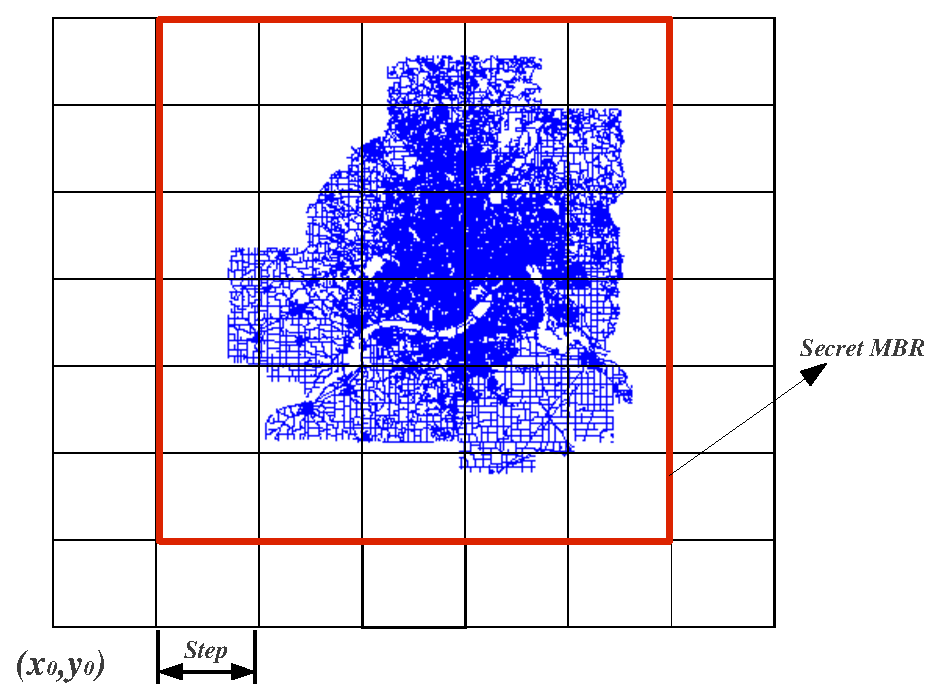
\epsfig{file=SecretGrid.eps,width=0.7\columnwidth}
\caption{Master Grid and MBR}
\label{fig:grid}
\end{figure}

\subsubsection{Secret Square Size}

The third secret key is an integer number $l$ that determines the size of a square box that we
used to select a small neighbourhood of road segments from which to compute the watermarks.
More details of the use of $l$ will be presented in \secref{sec:insert} and illustrated in
\figref{fig:insert}. 
%In insertion and detection parts of our algorithm, another two secret keys
%are applied. To determine the position to insert watermark of the selected points,
%we use a square centered at the selected data point with a secret side length to 
%choose the neighbourhood road segments. This process could be illustrated by Figure
%\ref{fig:13}. When hashing to get the target position, a secret random table is also used.


\subsection{Space Partitioning Algorithm}

This algorithm is used in both insertion and detection of the watermarks. 
This algorithm partitions the space bounded by the secret MBR for a map
recursively into small regions using a quadtree structure according to the 
density of the roads. Each node in the tree represents a subregion of the map.
The leaf node represents a region in which the total length of road segments
within is between $\theta$ and $4*\theta$ meters, where $\theta$ is a parameter of the algorithm. 
\figref{fig:quadtree} illustrate the quadtree created from partitioning an MBR
shown on the left. The detailed algorithm is listed in Algorithm \ref{Partition}.

%Leaf nodes represent those subregions that is partitioned in the deepest level. 
%Non-leaf nodes represent the areas consisting of all subareas represented by their children. In Figure \ref{fig:quadtree}, subregion one is partitioned two times, since its road density is greater. The second subregion is not partitioned since the road in it is more sparce.

\begin{figure}[th]
\centering
\epsfig{file=quadtree.eps,width=\columnwidth}
\caption{Quadtree}
\label{fig:quadtree}
\end{figure}

The partition algorithm must create roughly the same kind of segmentation
result on the same map, with or without watermarks, before or after attacks.
Our algorithm works because it uses length of roads per node to guide the 
partition process. Road length of an area cannot be changed arbitrarily
due to the constraints of perception tolerance which must be observed by both
the watermark producer and the attacker. No matter a watermarked map is cropped 
or merged with other parts from different maps, this method still produces 
almost the same partition results for the watermarked part. %\KZ{This paragraph is critical!}

Partition algorithm is the main part of both insertion
and detection algorithms. Time complexity $\T$ is related to number of edges 
$|E|$ in map and the ratio of partition threshold $\theta$ to total road length
$\LEN=\sum_{R \in M}length(R)$. $\theta$ should be a constant, which sets a threshold 
for the algorithm how much information a subregion should contain at least to embed 
a one bit watermark. Thus the time complexity is 
\[\T = O(|E|\log\LEN) \le O(|V|^2\log(\frac{\LEN}{\theta})).\]

%A digital road map $M$ is a special case of a connected graph 
%$G=\left\{V,~E\right\}$.
%A general connected graph has the following constraints on $|E|$ and $|V|$.
%\[|V|-1 \le |E|\le \frac{|V|(|V|-1)}{2}.\]
%which means in the worse case of a fully connected graph, 



However, in practice, map graphs are much more sparse. In fact, 
every vertex is either the end of a road, a turning point of a road or a junction. 
So the number of edges connected to a vertex is bounded by the maximum number of 
roads leading to a junction, which is a small number $q$ (typically $q \le 6$). 
That is,
\[|E| \le \frac{q|V|}{2}. \]
And therefore
\[\T = O(|V|\log\LEN).\]
%Considering the practical situation, the number of intersecting vertices is 
%insignificant comparing to $|E|$. On other hand, to control the cost, the
%intersecting vertices of roads in real world are also weakly connected. 
%Then we have a good reason to assume that $|E| \cong |V|$. 

%In algorithm \ref{Partition}, the secret MBR is generated from the master grid(see Figure \ref{fig:grid}). Then the map area is partitioned iteratively according to the density of roads such that finally the total road length included in every subregion has more than m meters and less than $4 * m$ meters. Finally, we output all of these subregions. Here we modify Quadtree by merging subregion with less roads with its smallest neighbour.

\begin{algorithm}[th]
\caption{Partition}
\label{Partition}
\begin{algorithmic}[1]
\Require
\State 	  $G$: Master grid 
\State    $M$: Original dataset
\State    $\theta$: Road length threshold
\Ensure
\State    $PO$: Subregion list
\State    $T$: Quadtree
\Function{PARTITION}{$G,~M,~T,~\theta$}
\State $L\leftarrow$new queue
\State $PO\leftarrow$new list
\State $T\leftarrow MBR(G,~M)$
\State $L.Push(T)$
\While{$L$ is not empty}
\State partition region $\R \leftarrow L.pop$ into ${\R}_{i}$, $i\in \left\{1,2,3,4\right\}$
\For{each ${\R}_{i}$}
\If{road length in ${\R}_{i} < \theta$}
\State merge ${\R}_{i}$ with its smaller neighbour
\ElsIf{road length in ${\R}_{i} > 4*\theta$}
\State $\R.children_i \leftarrow {\R}_{i}$ 
\State  $L.push(\R.children_i)$
\Else{}
\State $\R.children_i \leftarrow {\R}_{i}$
\State insert ${\R}_{i}$ to $PO$
\EndIf
\EndFor
\EndWhile\\
\Return $PO$
\EndFunction
\end{algorithmic}
\end{algorithm}


\subsection{Watermark Insertion Algorithm}
\label{sec:insert}

\begin{figure}[th]
\centering
\epsfig{file=insertion.eps,width=0.5\columnwidth}
\caption{Insertion Strategy %\KZ{I think in this fig you want draw a 
%dashed line circle
%centered at the center of the square box and this circle touches on P(x, y)
%to show how to find P(x, y)}
}
\label{fig:insert}
\end{figure} 


The insertion algorithm first generates a set of subregions by partitioning. 
Then it inserts one watermark into each subregion at the leaf nodes of the 
quadtree. The watermark is inserted into a road vertex $P(x, y)$ which is
closest to the center of the subregion (marked by the black box in 
\figref{fig:insert}). To compute the exact watermark to be inserted, the algorithm
then draw a square box of size $l$ (the other secret key) centered at
$P(x, y)$ (the red box in \figref{fig:insert}). Let $sl$ be the length of road
segments that intersects the square box, and let $j$ be a value hashed from
$sl$. We then set the $j^{th}$ least significant bit in $x$ coordinate of $P$ 
to ``1''. Details are in Algorithm \ref{Insertion}. Here we pay special
attention to the hash function in algorithm. This hash function should 
guarantee to hash a point $P$ before and after watermarking. If the watermarked map is 
attacked(some end points of those segments intersecting $Q$ is unfortunately changed),
this hash function should also hash to the same $j$. In fact, we design this 
function with a sensitive tolerance of possible distortion. Assume that the possible
great distortion of a single point is $J_{max}$ LSB of the coordinates.
\begin{eqnarray*}
j&=&Hash(Trans(sl),k)\\
Trans(x)&=& x \wedge \underbrace {11\ldots1\overbrace {00\ldots0}^{J_{max}} }_{L_{x} } 
\end{eqnarray*}
where $L_{x}$ is the bit length of $x$.
%\KZ{This hash function is critical. We need to show what exactly is this
%function. How can we make sure that it has the necessary tolerance to
%defeat possible distortion?} 

%
%To find the right vertex, we use a square of size $l$ centered at the selected data 
%point $P$ with a secret side length to choose the neighbourhood 
%road segments which interset the very square (see Figure \ref{fig:insert}). 
%In Algorithm \ref{Insertion}, we 
%Then data points closest to the center of subregions are selected to watermark. 
%We watermark the selected data points according to their neighbours in space. 
%Specifically, 
%Then we can summarize the total number of these segments and hash 
%it with a secret random table to a certain least significant bit (LSB) position. 
%Then we set the corresponding LSB value for the selected data point to be ``1''.

\begin{algorithm}[th]
\caption{Insert Watermark into Map}
\label{Insertion}
\begin{algorithmic}[1]
\Require
\State 	  $G$: Master grid 
\State    $M$: Original dataset
\State    $\theta$: Road length threshold
\State    $l$: Secret square size
\State    $k$: Secret hash key
\Ensure
\State     $M'$: Watermarked dataset
\Procedure{INSERTION}{$M',~M,~G,~l,~k,~\theta$}
\State $PO\leftarrow$ PARTITION( $G,~M,~NULL,~\theta$ )
\For{each region ${\R}_{i} \in PO$}
\If {road length in ${\R}_{i}>\theta$}
\State $P\leftarrow$ point closest to ${\R}_{i}.center$
\State draw a square $Q$ of side length $l$ centered at $P$
\State $sl \leftarrow$ length of line segments intersecting $Q$
\State j $\leftarrow$ Hash( $k,sl$ )
\State $j^{th}$ LSB of $P.x \leftarrow$ 1
\EndIf
\EndFor
\EndProcedure
\end{algorithmic}
\end{algorithm}

In Algorithm \ref{Insertion}, $PO$ is a list of $submap$. We can distinguish all
watermarking points by traversing it. Thus insertion computation complexity is
$\T+O(|V|)$.
\[\T_{insert} = O(|V|\log\LEN).\]

\subsection{Watermark Detection Algorithm}

In the detection part, we partition the map into smallest possible sub-regions
using the same strategy as insertion. Then we select the data points closest
to the center of the regions to detect whether the watermark exists there.
Each subregion which has been detected contain a watermark casts a vote
which collectively contributes to the final decision of whether a larger
area is watermarked as a whole.
In algorithm \ref{algo:Detection}, 
we partition the map that may have been attacked and select the data points to detect.
Then we calculate the total number of neighbour road segments and compute
the watermarked bit location in the same way as in the insertion 
algorithm. While selecting points, we construct the quadtree which depicts 
the whole digital map. For leaf nodes of the quadtree, if the bit value at 
the right position is ``1'', we mark this subregion as a ``match''. 


\begin{algorithm}[th]
\caption{Detect Watermark from a Suspicious Map}
\label{algo:Detection}
\begin{algorithmic}[1]
\Require
\State 	  $G$: Master grid 
\State    $M'$: Watermarked dataset
\State    $\theta$: Road length threshold
\State    $l$: Secret square size
\State    $k$: Secret hash key
\Ensure
\State    $Yes/No$
\Procedure{DETECTION}{$M,~G,~l,~k,~\theta$}
\State $T \leftarrow$ new Quadtree
\State $PO \leftarrow$ PARTITION( $G,~M,~\&T,~\theta$ )
\For{each region ${\R}_{i} \in PO$}
\If {road length in ${\R}_{i} > \theta$}
\State $P\leftarrow$ point closest to ${\R}_{i}.center$
\State draw a square $Q$ of side length $l$ center at $P$
\State $sl \leftarrow$ length of line segments intersecting $Q$
\State j $\leftarrow$ Hash( $k,sl$ )
\If {$j^{th}$ LSB of $P.x$ is 1}
\State Mark ${\R}_{i}$ as ``match''
\EndIf
\EndIf
\EndFor
\State MARK\_QUADTREE( $T$ )
\State DF\_TRAVERSE( $T$ )
\EndProcedure
\end{algorithmic}
\end{algorithm}

\begin{algorithm}[th]
\caption{Mark The Quadtree}
\label{algo:mark}
\begin{algorithmic}[1]
\Statex
\Function{MARK\_QUADTREE}{$T$}
\If{ $T$ isn't a leaf node}
\For{each $T_i\in T.children$}
\State MARK\_QUADTREE(${T}_{i}$)
\State $T$.match$\leftarrow$$T$.match+${T}_{i}$.match
\State $T$.total$\leftarrow$$T$.total+${T}_{i}$.total 
\EndFor
\Else{}
\If{The region of $T$ is ``match''}
\State $T$.match$\leftarrow$1
\Else{}
\State $T$.match$\leftarrow$0
\EndIf
\State $T$.total$\leftarrow$1
\EndIf\\
\Return
\EndFunction
\end{algorithmic}
\end{algorithm}



%It is obvious that the strategy of detection is similar to that of insertion. 
%We construct a Quadtree and get the knowledge 
%that whether its leaf nodes are `match' or not. 
To detect whether a part of a map contains the watermarks, we implement a 
function MARK\_QUADTREE($T$) to mark the whole quadtree 
(see Algorithm \ref{algo:mark}). The non-leaf nodes are marked according to the
``votes'' by the leaf nodes. For each node of quadtree, 
``total'' represents the total number of leaf nodes rooted at this node
and ``match'' represents the number of those leaf nodes which match.
Finally, we calculate the ratio of the number of leaf nodes that 
``match'' to the total number of leaf nodes of this subregion. 
If this ratio is greater than a predefined threshold, 
we conclude that this subregion of the map contains the watermark.
If the watermarked map is attacked by ``massive crop'' attack, 
the quadtree structure partitioned by detection algorithm will be 
just part of the insertion quadtree. 
However, it will be almost the same as the corresponding part of the quadtree 
for the whole map. 
The whole detection process is illustrated in Figure \ref{fig:detect}. 
Assuming that the shadow parts of sub-figure (a) is 
cropped from the watermarked map, 
the corresponding quadtree looks like the one in sub-figure (b).

\begin{figure}[h]
\centering
\epsfig{file=detection.eps,width=0.8\columnwidth}
\caption{Detection Strategy}
\label{fig:detect}
\end{figure} 

If the watermarked map is attacked by ``Merge Attack'', 
the detection quadtree will be almost the same as the insertion one. 
However, we can find the watermark only in part of the quadtree. 
In this case, the algorithm reports the sub-regions that are watermarked.
We can make a depth-first traversal of the detection quadtree to 
find the largest watermarked region (see Algorithm \ref{algo:find}).

\begin{algorithm}[th]
\caption{Find the Watermarked Region}
\label{algo:find}
\begin{algorithmic}[1]
\Statex
\Function{DF\_TRAVERSE}{$T$}
\If{ $conf(T) > \xi $}
\State $T$ is $Yes$
\Else{}
\For{each${T}_{i}\in T.children$}
\State DF\_TRAVERSE(${T}_{i}$)
\EndFor
\EndIf\\
\Return
\EndFunction
\Statex
\end{algorithmic}
\end{algorithm}

Computation complexity of Algorithm \ref{algo:Detection} is samilar to Algorithm \ref{Insertion}.
  
\[\T_{detec} = O(|V|\log\LEN).\]

\subsection{Detection Confidence}
In order to distinguish data with a watermark from data without a watermark, 
a watermarking process must guarantee a low false positive rate. 
%That means that it should maintain low rate of detecting 
%unwatermarked data as watermarked data. 
In our watermarking scheme, the data 
points we select to insert watermark may originally be ``1'' at the specified bit
position, so it is possible for the algorithm to detect an unwatermarked map 
as ``illegal''. We have to take the ``False Positive Probability'' 
as detection confidence. 
Since the watermarks are inserted at an arbitrary (hashed) bit position of
a vertex's x-coordinate, that bit can be either ``0'' or ``1'' with almost
equal probability. Therefore we define the detection confidence for a subregion
$\R$ as
%?gThe insertion algorithm selects the points to watermark according to 
%?gdensity of the road segments which is  and assuming that the road density thus we have a good reason to assume that the 
%?gprobability of specified bit to be ``1'' is roughly 50\%. 
%?gAnd it is independent for different points. In this case, the 
%?gFalse Positive Probability can be defined as:
\[
\label{pe}
conf (\R) ={ \sum _{ i=n }^{ N }{{N \choose i} {({ 1 }/{ 2 })}^{ N-i } { ({ 1 }/{ 2 }) }^{ i } }  }
\]
where $N$ is the total number of leaf nodes in $\R$
and $n$ is the number of leaf nodes which match. 
So whenever the detection confidence is larger than a predefined threshold, 
we conclude that this subregion is watermarked.



%%% Local Variables:
%%% mode: latex
%%% TeX-master: "paper"
%%% End:
%%% Local Variables:
%%% mode: latex
%%% TeX-master: "paper"
%%% End:
